\documentclass[14pt]{beamer}
\usepackage{./Estilos/BeamerUVM}
\usepackage{./Estilos/ColoresLatex}
\input{Preambulos/preambulo_Beamer_Madrid_default}
% \usefonttheme{serif}
\usepackage[clock]{ifsym}

\sisetup{per-mode=symbol}
\resetcounteronoverlays{saveenumi}

\title{\Large{Cinemática} \\ \normalsize{Física 1}}
\date{3 de julio de 2023}

\begin{document}
\maketitle

\section*{Contenido}
\frame{\frametitle{Contenido} \tableofcontents[currentsection, hideallsubsections]}


\section{Trabajo de desarrollo}
\frame{\tableofcontents[currentsection, hideothersubsections]}
\subsection{Indicaciones}

\begin{frame}
\frametitle{Trabajo de desarrollo}
Deberás de realizar un trabajo con los siguientes puntos:
\pause
\setbeamercolor{item projected}{bg=bananayellow,fg=ao}
\setbeamertemplate{enumerate items}{%
\usebeamercolor[bg]{item projected}%
\raisebox{1.5pt}{\colorbox{bg}{\color{fg}\footnotesize\insertenumlabel}}%
}
\begin{enumerate}[<+->]
\item Un revisión biográfica de Isaac Newton y de Johannes Kepler.
\seti
\end{enumerate}
\end{frame}
\begin{frame}
\frametitle{Trabajo de desarrollo}
\setbeamercolor{item projected}{bg=bananayellow,fg=ao}
\setbeamertemplate{enumerate items}{%
\usebeamercolor[bg]{item projected}%
\raisebox{1.5pt}{\colorbox{bg}{\color{fg}\footnotesize\insertenumlabel}}%
}
\begin{enumerate}[<+->]
\conti
\item Para Isaac Newton deberás de presentar de manera general, las aportaciones que hizo para la mecánica, en particular, las llamadas Leyes de Newton, respondiendo ¿de qué manera logró establecer o construir esas leyes?
\seti
\end{enumerate}
\end{frame}
\begin{frame}
\frametitle{Trabajo de desarrollo}
\setbeamercolor{item projected}{bg=bananayellow,fg=ao}
\setbeamertemplate{enumerate items}{%
\usebeamercolor[bg]{item projected}%
\raisebox{1.5pt}{\colorbox{bg}{\color{fg}\footnotesize\insertenumlabel}}%
}
\begin{enumerate}[<+->]
\conti
\item Para Johannes Kepler, presentarás su trabajo conocido como las Leyes de Kepler, ¿en qué consisten? ¿qué fenómenos explican?
\seti
\end{enumerate}
\end{frame}
\begin{frame}
\frametitle{Trabajo de desarrollo}
\setbeamercolor{item projected}{bg=bananayellow,fg=ao}
\setbeamertemplate{enumerate items}{%
\usebeamercolor[bg]{item projected}%
\raisebox{1.5pt}{\colorbox{bg}{\color{fg}\footnotesize\insertenumlabel}}%
}
\begin{enumerate}[<+->]
\conti
\item Para entender las Leyes de Kepler, será necesario estudiar también el lugar geométrico llamado elipse. Pero no desde el punto de vista matemático, es decir, no hay que señalar la ecuación que la define, sino las propiedades o características que presenta una elipse.
\seti
\end{enumerate}
\end{frame}
\begin{frame}
\frametitle{Trabajo de desarrollo}
\setbeamercolor{item projected}{bg=bananayellow,fg=ao}
\setbeamertemplate{enumerate items}{%
\usebeamercolor[bg]{item projected}%
\raisebox{1.5pt}{\colorbox{bg}{\color{fg}\footnotesize\insertenumlabel}}%
}
\begin{enumerate}[<+->]
\conti
\item Deberás de presentar un método a partir del cual se puede construir una elipse en el cuaderno. Hay varias propuestas, pero la que elijas, deberás de presentar el desarrollo completo, de tal manera que muestres la manera en la que se obtiene.
\seti
\end{enumerate}
\end{frame}
\begin{frame}
\frametitle{Trabajo de desarrollo}
\setbeamercolor{item projected}{bg=bananayellow,fg=ao}
\setbeamertemplate{enumerate items}{%
\usebeamercolor[bg]{item projected}%
\raisebox{1.5pt}{\colorbox{bg}{\color{fg}\footnotesize\insertenumlabel}}%
}
\begin{enumerate}[<+->]
\conti
\item Esta actividad de desarrollo aportará hasta $10$ puntos de evaluación continua.
\item La evaluación se hará con una rúbrica, pero el nivel de calidad y exigencia del trabajo será mayor.
\seti
\end{enumerate}
\end{frame}
\begin{frame}
\frametitle{Trabajo de desarrollo}
\setbeamercolor{item projected}{bg=bananayellow,fg=ao}
\setbeamertemplate{enumerate items}{%
\usebeamercolor[bg]{item projected}%
\raisebox{1.5pt}{\colorbox{bg}{\color{fg}\footnotesize\insertenumlabel}}%
}
\begin{enumerate}[<+->]
\conti
\item La entrega del trabajo será por Teams, el plazo para el envío es el día 5 de julio a las 8 pm.
\item No se recibirán trabajos extemporáneos, a menos que se presente la evidencia de problemas técnicos durante el envío y que se haya notificado oportunamente a la Coordinación Académica y al Profesor.
\end{enumerate}
\end{frame}

\section{Ejercicios de recuperación}
\frame{\tableofcontents[currentsection, hideothersubsections]}
\subsection{Trabajo a resolver}

\begin{frame}
\frametitle{Objetivo del Trabajo}
Con la finalidad de apoyar en la recuperación del promedio para los siguientes exámenes parciales, \pause se dejarán una serie de \textocolor{red}{ejercicios adicionales} para Evaluación Continua.
\end{frame}
\begin{frame}
\frametitle{Ejercicios opcionales}
Estos ejercicios serán de carácter \textocolor{cobalt}{opcional}, \pause es decir, la alumna o alumno que desee resolverlos y enviarlos, les sumará $5$ puntos adicionales a la Evaluación Continua.
\end{frame}
\begin{frame}
\frametitle{Puntaje adicional}
Si por ejemplo, para el segundo parcial se tienen 20 puntos de Evaluación Continua, \pause al sumar $5$ puntos adicionales, el puntaje se calculará sobre los $20$ ejercicios, \pause por decir: \pause $25/20$ de puntaje.
\end{frame}
\begin{frame}
\frametitle{Puntaje y calificación de teoría}
Ese puntaje de Evaluación Continua corresponde al $50\%$ de la calificación de teoría, \pause lo que ayudaría a subir el promedio del segundo parcial.
\end{frame}
\begin{frame}
\frametitle{Ventaja para la calificación}
Quien desee resolver y enviar los ejercicios, podrá mejorar su promedio para el siguiente parcial.
\\
\bigskip
Lo que es completamente atractivo para mejorar la calificación del curso.
\end{frame}
\begin{frame}
\frametitle{Fecha de entrega}
Los ejercicios adicionales se dejarán cada semana, \pause debiendo de entregarse el día domingo a las 8 pm.
\end{frame}
\begin{frame}
\frametitle{Aviso importante}
Los ejercicios adicionales NO sustituyen a los ejercicios de Evaluación Continua que se dejarán.
\\
\bigskip
\pause
Si alguien decide no enviar los ejercicios adicionales, no tendrá penalización alguna.
\end{frame}

\section{Cinemática}
\frame{\tableofcontents[currentsection, hideothersubsections]}
\subsection{Conceptos}

\begin{frame}
\frametitle{¿Qué es la mecánica?}
La \textocolor{ao}{mecánica} es la rama de la Física que se encarga del estudio de los cuerpos en movimiento; \pause se divide en \pause \textocolor{burgundy}{cinemática} \pause y \textocolor{darkgreen}{dinámica}.
\end{frame}
\begin{frame}
\frametitle{Cinemática}
La cinemática es la parte de la mecánica que estudia los diferentes tipos de movimiento de los objetos sin atender las causas que lo produjeron.
\end{frame}
\begin{frame}
\frametitle{Movimiento}
Es el cambio de lugar que experimenta un cuerpo dentro de un espacio determinado.
\end{frame}
\begin{frame}
\frametitle{Sistema de referencia}
Sistema de elementos que sirve para fijar la posición de un cuerpo en movimiento.
\end{frame}
\begin{frame}
\frametitle{Posición}
Es el lugar físico en el que se encuentra un cuerpo dentro de un espacio determinado.
\end{frame}
\begin{frame}
\frametitle{Distancia}
La distancia recorrida por un móvil es una \textocolor{magenta}{magnitud escalar}, \pause ya que sólo interesa saber cuál fue la magnitud de la longitud recorrida por el móvil durante la trayectoria seguida, sin importar en qué dirección lo hizo.
\end{frame}
\begin{frame}
\frametitle{Trayectoria}
Es la línea que une las diferentes posiciones que a medida que pasa el tiempo va ocupando un punto en el espacio o, de otra forma, es el camino que sigue el objeto dentro de un movimiento.
\end{frame}
\begin{frame}
\frametitle{Trayectoria}
\begin{figure}
    \centering
    \includegraphics[scale=0.45]{Imagenes/Trayectoria_01.png}
\end{figure}
\end{frame}
\begin{frame}
\frametitle{Tipos de Trayectoria}
Cuando la trayectoria es una línea recta se dice que el movimiento es rectilíneo.
\\
\bigskip
\pause
Cuando la trayectoria es un círculo decimos que el movimiento es circular.
\end{frame}
\begin{frame}
\frametitle{Desplazamiento}
El desplazamiento de un móvil es una \textocolor{cerise}{magnitud vectorial}, ya que corresponde a una distancia medida en una dirección particular entre dos puntos: el de partida y el de llegada.
\end{frame}
\begin{frame}
\frametitle{Desplazamiento}
\begin{figure}
    \centering
    \includegraphics[scale=0.45]{Imagenes/Trayectoria_02.png}
\end{figure}
\end{frame}

\section{Movimiento Rectilíneo Uniforme}
\frame{\tableofcontents[currentsection, hideothersubsections]}
\subsection{Conceptos relevantes}

\begin{frame}
\frametitle{Rapidez}
La \textocolor{auburn}{rapidez} es la distancia recorrida por un objeto en cierto tiempo.
\\
\bigskip
\pause
Es una \textocolor{awesome}{cantidad escalar}, porque se define con una magnitud y una unidad de medida.
\end{frame}
\begin{frame}
\frametitle{Expresión para la rapidez}
La rapidez se obtiene mediante la siguiente expresión:
\pause
\begin{align*}
\text{rapidez} = \dfrac{\text{distancia}}{\text{tiempo}}
\end{align*}
Las unidades son metros por segundo (\unit[per-mode=symbol]{\meter\per\second})
\end{frame}
\begin{frame}
\frametitle{Velocidad}
Es la razón de cambio del desplazamiento de un objeto con respecto al tiempo.
\\
\bigskip
\pause
La velocidad es una \textocolor{byzantine}{magnitud vectorial}.
\end{frame}
\begin{frame}
\frametitle{Expresión para la velocidad}
La velocidad se obtiene mediante la siguiente expresión:
\pause
\begin{eqnarray*}
\begin{aligned}
\text{velocidad} = \dfrac{\text{desplazamiento}}{\text{tiempo}} \pause \hspace*{1.5cm} v = \dfrac{d}{t}
\end{aligned}
\end{eqnarray*}
\pause
Las unidades de la velocidad son metros por segundo (\unit[per-mode=symbol]{\meter\per\second})
\end{frame}
\begin{frame}
\frametitle{Velocidad final}
Es el último instante o momento de la distancia recorrida en el tiempo.
\end{frame}
\begin{frame}
\frametitle{Velocidad media}
Promedio de la suma de todas las distancias y tiempos recorridos.
\end{frame}
\begin{frame}
\frametitle{El triángulo de la velocidad}
En física es común apoyarse con ciertas reglas de tipo visual, que nos ayudarán a simplificar el manejo de una expresión.
\\
\bigskip
\pause
Tal es el caso del \textbf{Triángulo de la velocidad}.
\end{frame}
\begin{frame}
\frametitle{El triángulo de la velocidad}
\begin{figure}
\centering
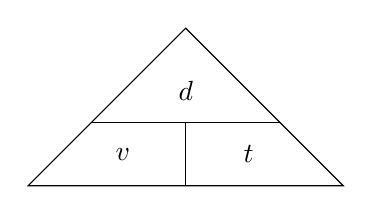
\begin{tikzpicture}
    \draw (0, 0) -- (4, 0) -- (2, 2) -- cycle;
    \draw (2, 0) -- (2, 0.8);
    \draw (0.8, 0.8) -- (3.2, 0.8);

    \node at (2, 1.2) {$d$};
    \node at (1.2, 0.4) {$v$};
    \node at (2.8, 0.4) {$t$};
\end{tikzpicture}
\end{figure}
La idea con esta imagen es recuperar de la expresión, la operación que se necesite si nos piden alguna de las tres variables.
\end{frame}
\begin{frame}
\frametitle{Ejercicio de velocidad}
Un corredor avanza \SI{2}{\kilo\meter} en un tiempo de \SI{15}{\minute}.
\\
\bigskip
\pause
Calcula su velocidad en \unit[per-mode=symbol]{\kilo\meter\per\hour} y en \unit[per-mode=symbol]{\meter\per\second}.
\pause
Revisa que nos piden hacer una conversión de unidades.
\end{frame}
\begin{frame}
\frametitle{Primer paso para la solución al ejercicio}
Se recomienda siempre tener los \textocolor{red}{datos} que nos indica el enunciado.
\pause
\begin{eqnarray*}
\begin{aligned}
\text{desplazamiento} &= \SI{2}{\kilo\meter} \\[0.5em] \pause
\text{tiempo} &= \SI{15}{\minute}
\end{aligned}
\end{eqnarray*}
\end{frame}
\begin{frame}
\frametitle{Segundo paso para la solución al ejercicio}
Nos conviene anotar la \textocolor{cadmiumgreen}{expresión} a utilizar, ya sea de uso directo o tengamos que despejar alguna variable. \pause Nos apoyamos con el triángulo de la velocidad:
\pause
\begin{figure}
\centering
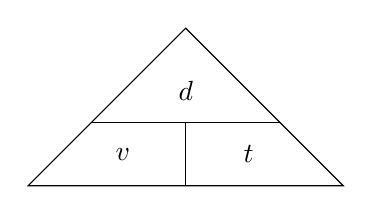
\begin{tikzpicture}
    \draw (0, 0) -- (4, 0) -- (2, 2) -- cycle;
    \draw (2, 0) -- (2, 0.8);
    \draw (0.8, 0.8) -- (3.2, 0.8);

    \node at (2, 1.2) {$d$};
    \node at (1.2, 0.4) {$v$};
    \node at (2.8, 0.4) {$t$};
\end{tikzpicture}
\end{figure}        
\end{frame}
\begin{frame}
\frametitle{Tercer paso para la solución al ejercicio}
Hacemos la sustitución con los valores que nos indica el enunciado:
\pause
\begin{eqnarray*}
\begin{aligned}
v = \dfrac{\SI{2}{\kilo\meter}}{\SI{15}{\minute}} = \pause \SI[per-mode=fraction]{0.1333}{\kilo\meter\per\minute}
\end{aligned}
\end{eqnarray*}
\pause
Nos falta hacer la conversión de unidades.
\end{frame}
\begin{frame}
\frametitle{Haciendo la conversión de unidades}
\begin{eqnarray*}
\begin{aligned}
v &= \SI[per-mode=fraction]{0.1333}{\kilo\meter\per\minute} \left( \dfrac{\SI{60}{\minute}}{\SI{1}{\hour}} \right) = \pause \SI[per-mode=fraction]{8}{\kilo\meter\per\hour} \\[0.5em] \pause
v &= \SI[per-mode=fraction]{0.1333}{\kilo\meter\per\minute} \left( \dfrac{\SI{d3}{\meter}}{\SI{1}{\kilo\meter}} \right) \left( \dfrac{\SI{1}{\hour}}{\SI{3.6d2}{\second}} \right)  = \pause \SI[per-mode=fraction]{2.22}{\meter\per\second}
\end{aligned}
\end{eqnarray*}
\end{frame}
\begin{frame}
\frametitle{Otro ejercicio}
Un ciclista puede alcanzar en una bajada una velocidad de hasta \SI{35}{\kilo\meter\per\hour}.
\\
\bigskip
\pause
¿Qué distancia recorre en una pendiente después de \SI{2}{\minute}?
\end{frame}
\begin{frame}
\frametitle{Datos del enunciado}
\begin{eqnarray*}
\begin{aligned}
v &= \SI{35}{\kilo\meter\per\hour} \\[0.5em] \pause
t &= \SI{2}{\minute} \\[0.5em] \pause
d &= \, ?
\end{aligned}
\end{eqnarray*}
\end{frame}
\begin{frame}
\frametitle{Expresión a utilizar}
\begin{figure}
\centering
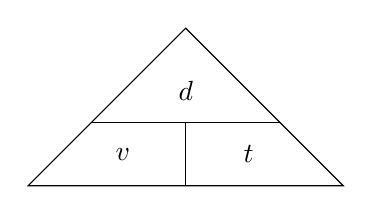
\begin{tikzpicture}
    \draw (0, 0) -- (4, 0) -- (2, 2) -- cycle;
    \draw (2, 0) -- (2, 0.8);
    \draw (0.8, 0.8) -- (3.2, 0.8);

    \node at (2, 1.2) {$d$};
    \node at (1.2, 0.4) {$v$};
    \node at (2.8, 0.4) {$t$};
\end{tikzpicture}
\end{figure}        
\begin{align*}
d = v \, t
\end{align*}
\end{frame}
\begin{frame}
\frametitle{Conversión de unidades}
Antes de hacer la sustitución, debemos de hacer una conversión de unidades para mantener la congruencia con el resultado:
\pause
\begin{eqnarray*}
\begin{aligned}
\SI[per-mode=fraction]{35}{\kilo\meter\per\hour} \left( \dfrac{\SI{d3}{\meter}}{\SI{1}{\kilo\meter}} \right) \left( \dfrac{\SI{1}{\hour}}{\SI{60}{\minute}} \right) = \pause \SI[per-mode=fraction]{583.3}{\meter\per\minute}
\end{aligned}
\end{eqnarray*}
\end{frame}
\begin{frame}
\frametitle{Conversión de unidades}
Ahora sustituimos los valores que ya hemos convertido:
\pause
\begin{eqnarray*}
\begin{aligned}
d &= v \, t \pause = \left( \SI[per-mode=fraction]{583.3}{\meter\per\minute} \right) \left( \SI{2}{\minute} \right) = \\[0.5em] \pause
d &= \SI{1166.6}{\meter}
\end{aligned}
\end{eqnarray*}
\end{frame}

\end{document}